\section{AI 工作区}

前面各节讲的是人怎么操作采析绘。这一章讲另一个角色。AI 工作区是右侧常驻的一块面板，它能读当前画布、数据集与运行记录，能调用只读工具，也能替你起草工作流。它和聊天框最大的区别在于写操作。凡是要改动你的东西，它只给一份提案，由你点应用才生效。

把它当成一个熟悉项目的助手，而不是一个替你做决定的开关。下面按第一次上手的顺序走，从打开面板到让 AI 读数据、管会话、盯运行。

\subsection{打开面板与三列布局}

菜单条点\texttt{AI 工作区}，右侧升起常驻面板。面板顶上一行是会话名、供应商与几个图标，下面是一个输入区。展开以后你能看到三列，从左到右是会话、对话、上下文与代理轨迹。日常屏幕宽度下第三列收起，点顶栏的全屏图标才展开，这样对话区能宽一些。图里是一份刚打开的空工作区，欢迎语下面五个按钮是系统给的示例问题，点一个就把它填进输入框。

\begin{figure}[H]\centering
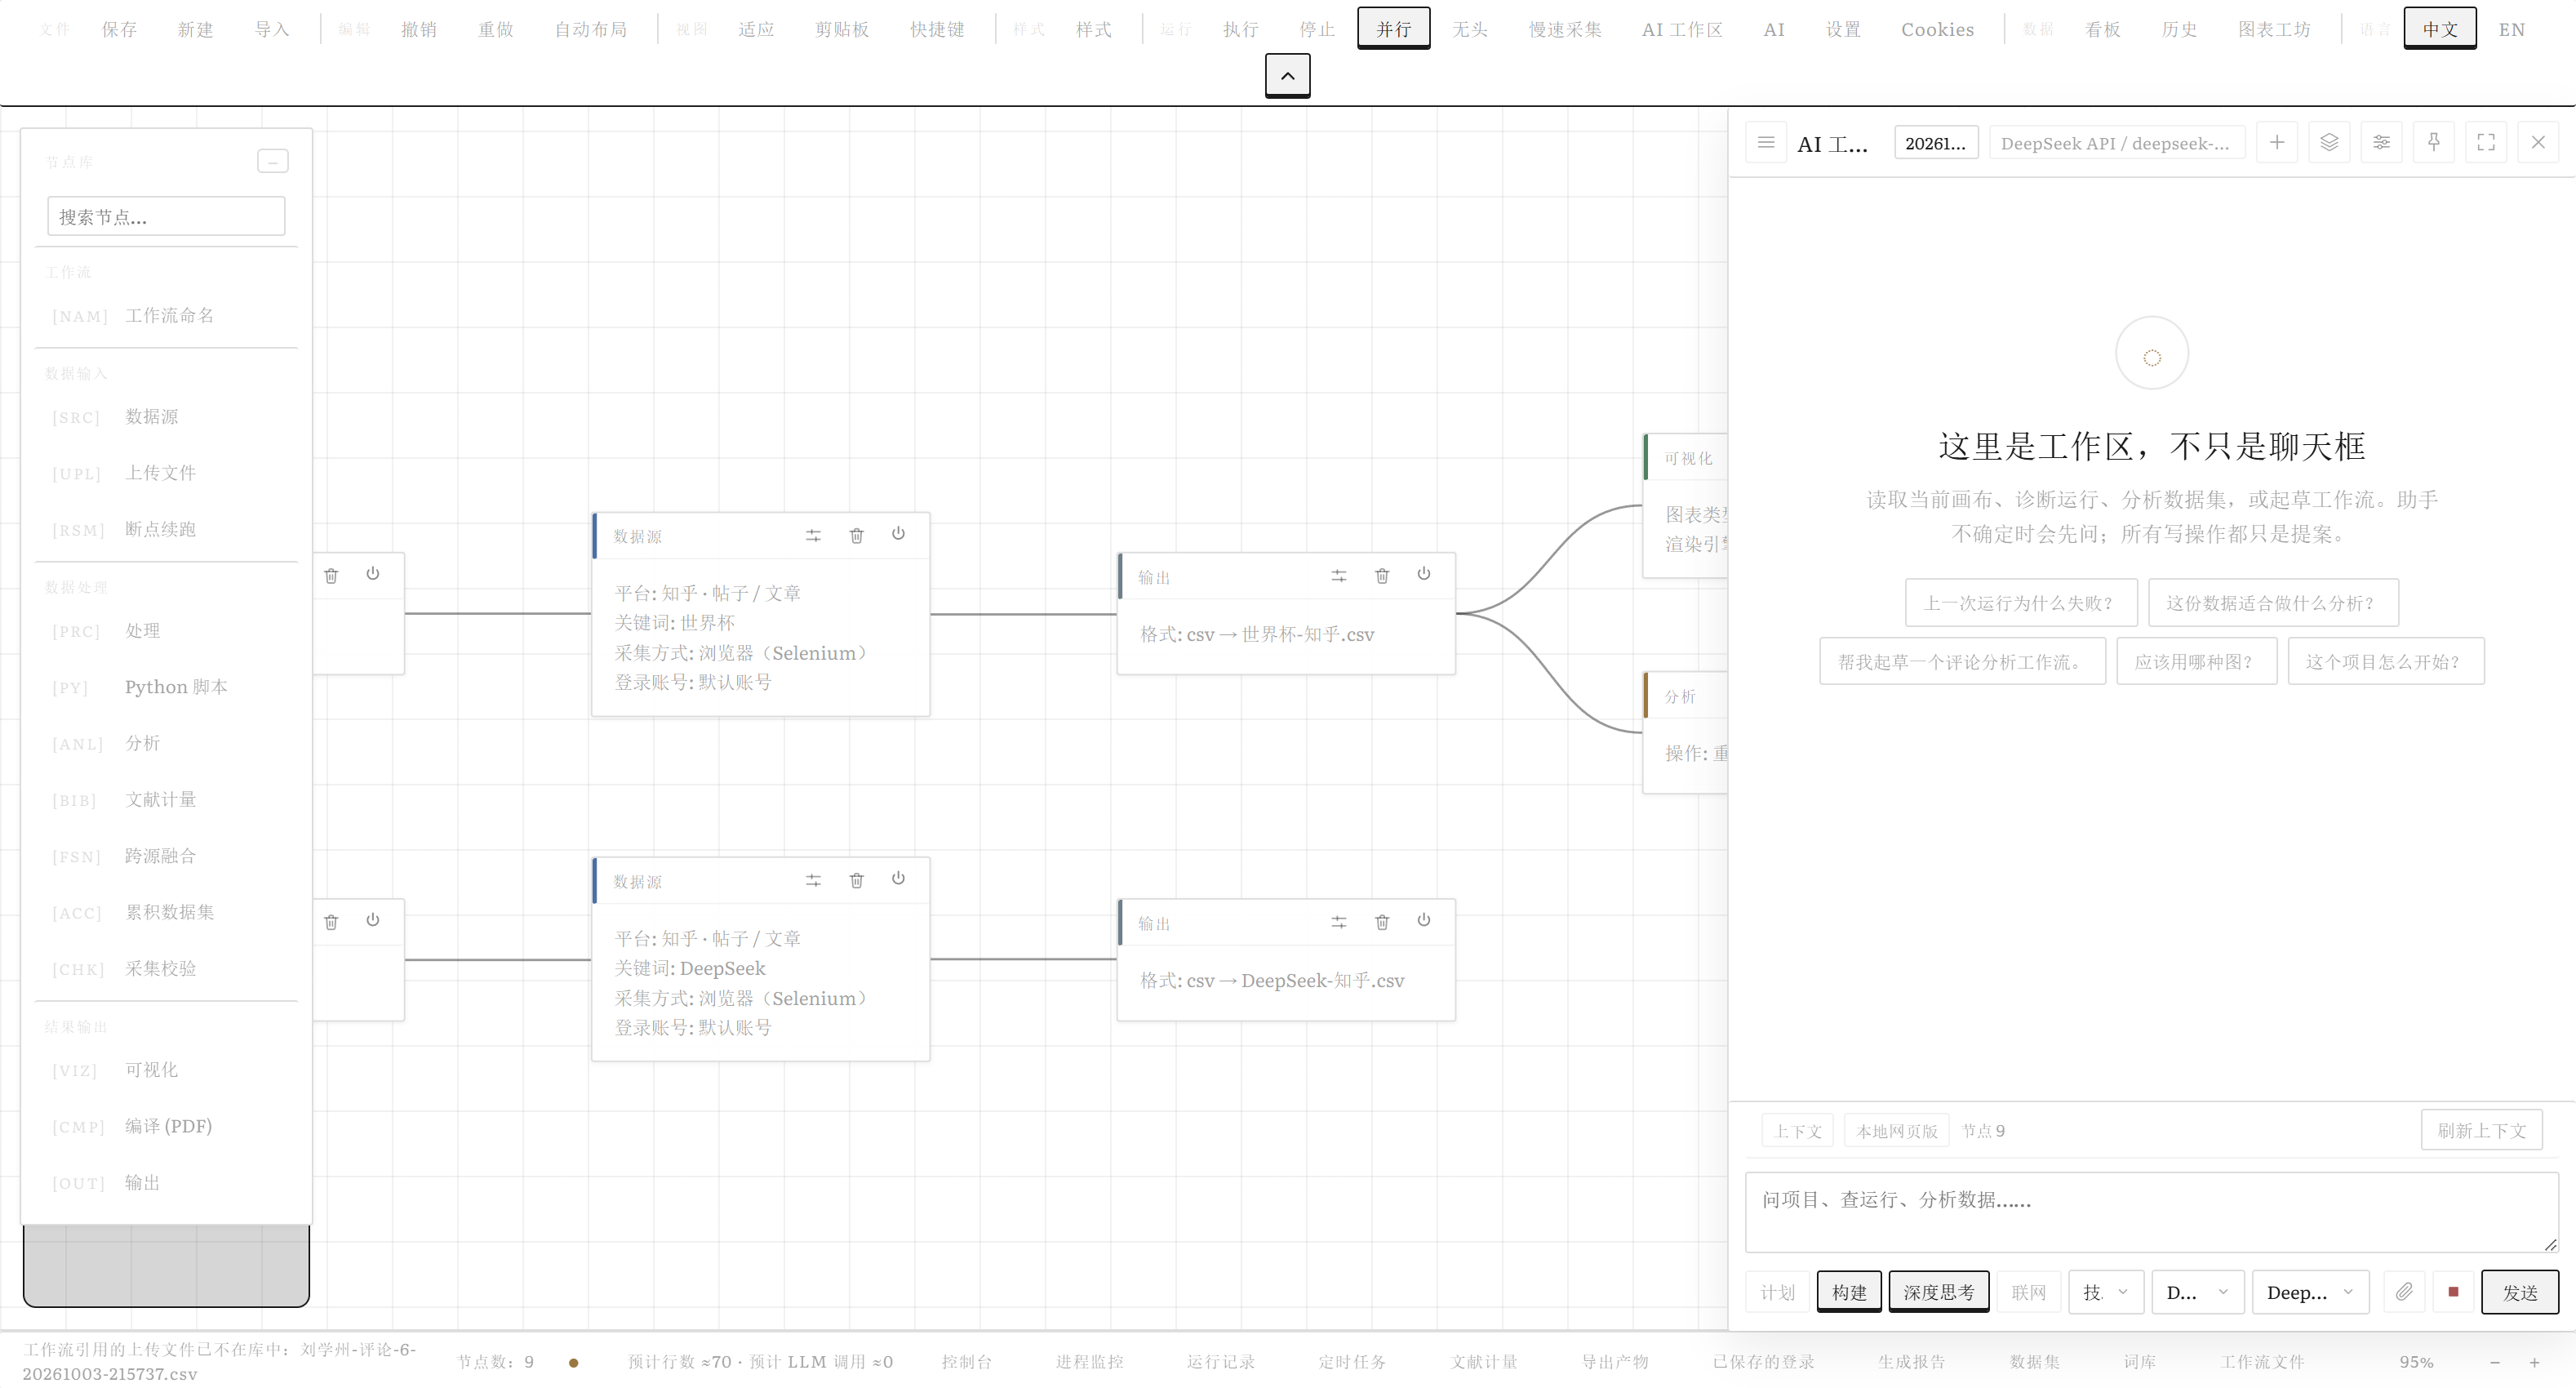
\includegraphics[width=0.98\textwidth]{ai-workspace.png}
\caption{AI 工作区的会话、对话、上下文三列与输入区}
\label{fig:ai-workspace}
\end{figure}

面板里所有词都跟着中英切换一起变，和画布共用一套语言设置。关掉面板再打开，上次聊到哪一条还在。

\subsection{第一次提问}

第一次用要先告诉它找谁说话。按下面的顺序做一遍。

\begin{enumerate}
\item 点供应商那一栏，或者打开顶栏的供应商设置。面板会列出四种调用方式。DeepSeek API 走原生协议，带深度思考、联网搜索、读链接与文件上传。OpenCode Go 与 OpenRouter 走通用协议。本地 Ollama 用你自己机器上的模型，不要钱也不联网，但要显存。云端模式下这一项会被按名字拒绝。
\item 选中一家以后在 API Key 输入框里填密钥，在模型下拉里挑一个，点测试连接看通不通，最后点保存。图里是 DeepSeek 的设置页。密钥只存在这个浏览器里，服务端只在一次请求内拿着它，不会写进数据库或日志。换一台机器要重新填一次。
\item 回到对话，在输入框里写问题。不知道问什么就点欢迎语下面的示例。第一次可以先问\texttt{这个项目怎么开始}。
\item 点发送。对话区出现一行生成中，旁边有秒数在跳，阶段词会随状态换。正常生成时写生成中，工具在跑时写等待采析绘返回，模型十五秒没吐字节时写模型还没返回内容。这一行只由真正的结束事件收掉。连接中途断了会明说上面可能不完整，不会让半截回答冒充完成。
\item 等它答完。按停止可以随时打断，停下时本轮启动的命令与后台任务一起中止，已经写出的半截回答留在转录里，刷新后是一行中性提示而不是红色报错。生成期间输入框仍可打字，重复点发送只会得到一句提示。
\end{enumerate}

\begin{figure}[H]\centering
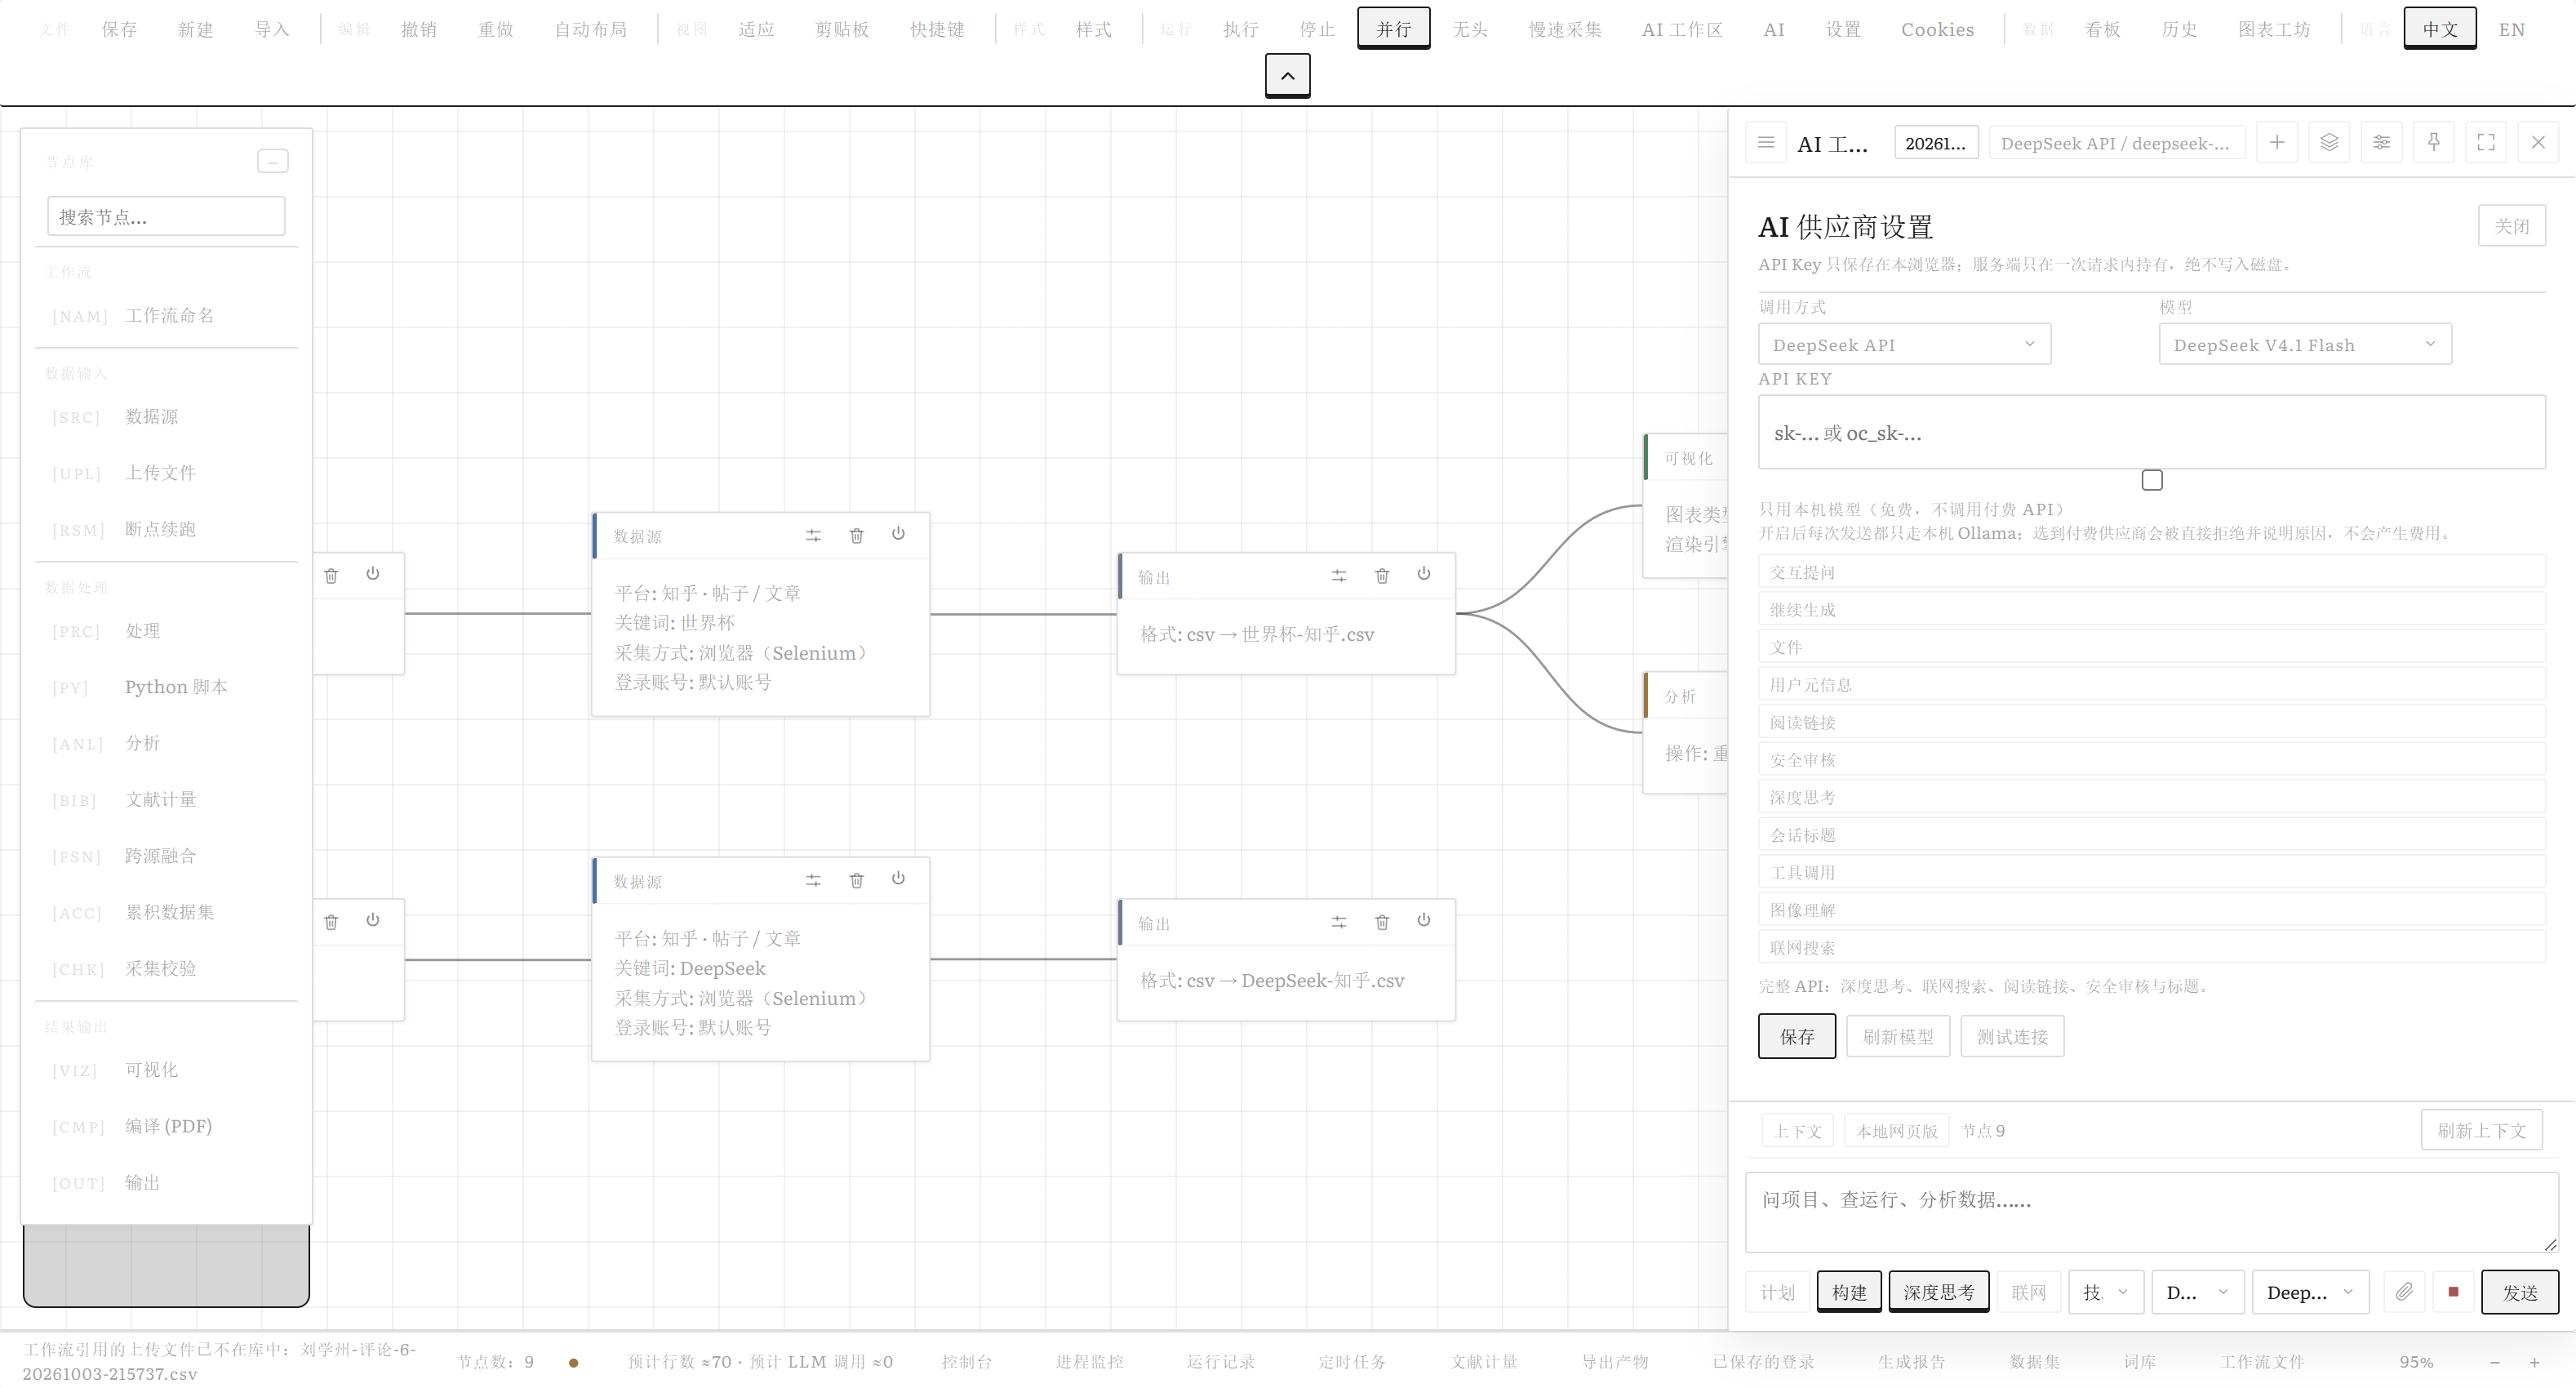
\includegraphics[width=0.98\textwidth]{ai-settings.png}
\caption{供应商设置里调用方式、密钥、模型与能力清单}
\label{fig:ai-settings}
\end{figure}

答完以后看它怎么写的。一轮完整的历史按顺序分成几块。技能行说明这一轮用了哪个技能，是自动路由还是你手选的。深度思考是模型的思考正文，点开才看。工具卡记着工具名、参数与返回结果，点开能看细节。计划是它给的步骤。回答在最后。刷新页面以后，同一份历史按同样顺序重画，不会只剩一段光秃秃的结论。

\subsection{管好会话}

每一次对话是一条会话。顶栏的三横线图标打开会话列，图里是它展开的样子。列顶有搜索框，按标题在服务端筛选，会话多的时候比翻列表快。新建会话从加号开始。一条会话可以置顶、归档、恢复和下载。下载给两种格式，Markdown 把对话排成一篇文档，JSON 原样保留每个存储块。

\begin{figure}[H]\centering
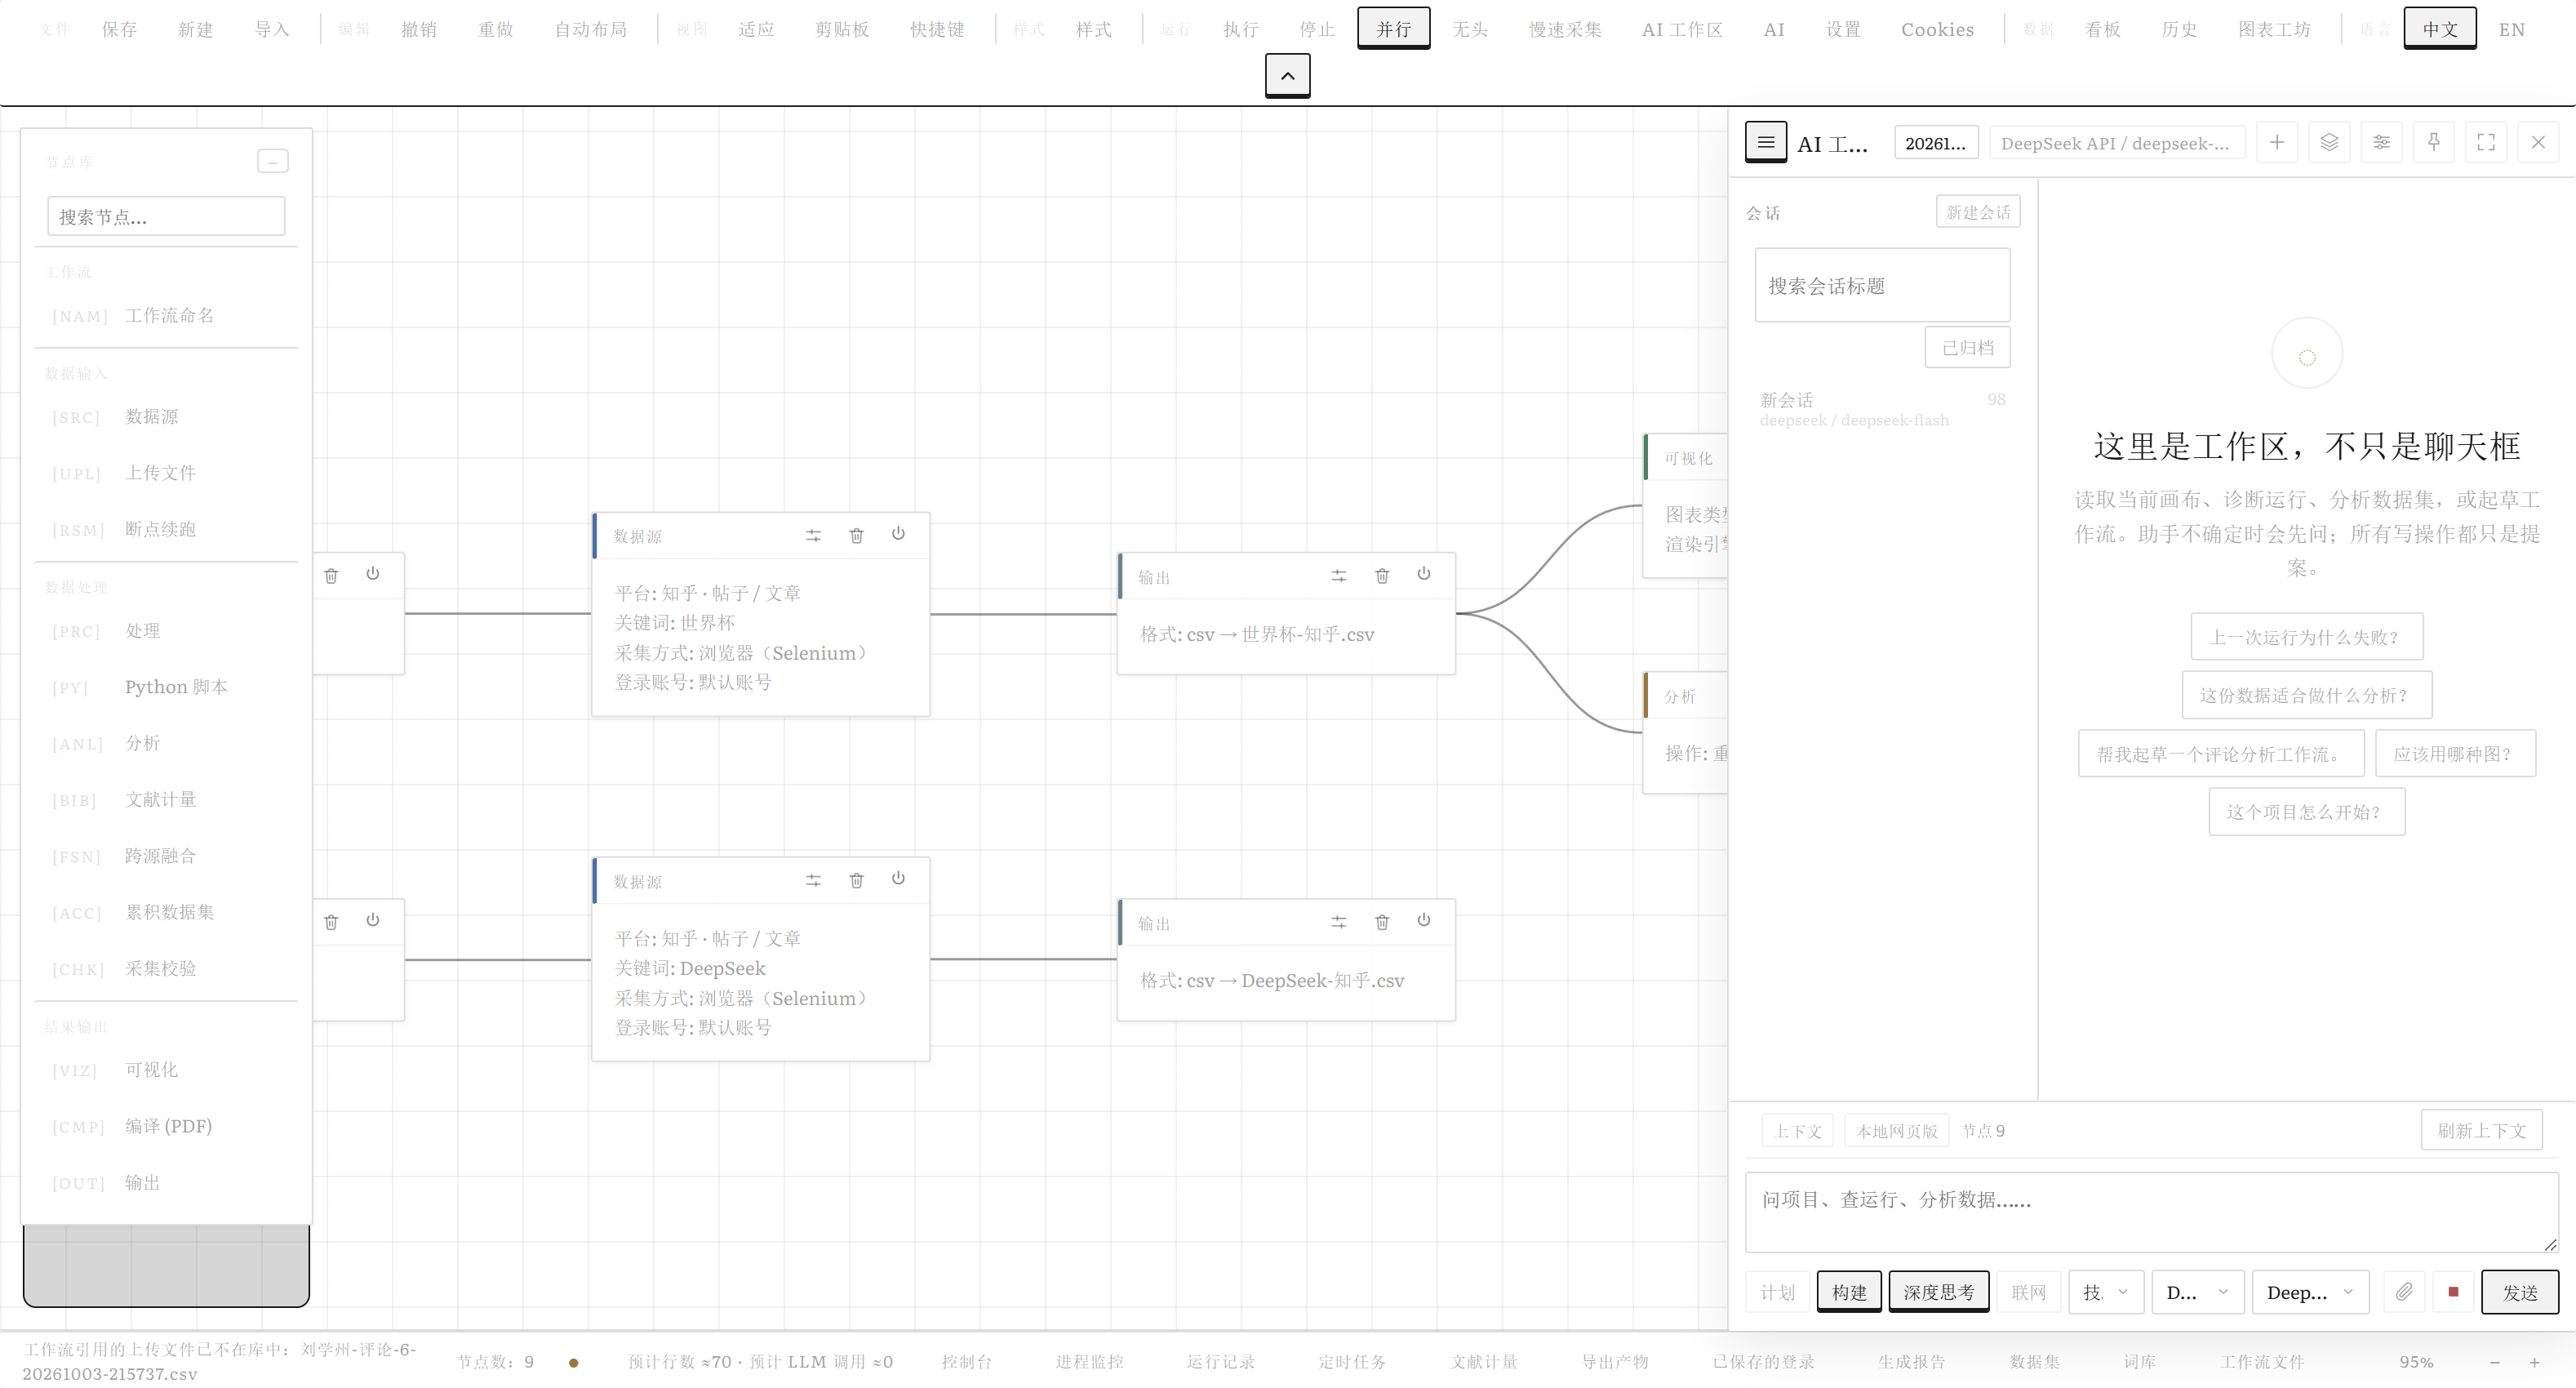
\includegraphics[width=0.98\textwidth]{ai-sessions.png}
\caption{会话列的搜索、新建、归档与会话条目}
\label{fig:ai-sessions}
\end{figure}

刷新页面会自动回到上次打开的那条会话。报错文字与还没回答的问题也一起存着，重开会话后仍在，不会因为刷新就丢掉。

\subsection{看它到底发了什么}

助手能看到多少东西，是由上下文决定的。输入区上面那条细栏写着当前宿主与画布节点数。要看真正发出去的文本，先点顶栏的全屏图标，再点第三列里的\texttt{查看将发送的上下文}，图里就是展开后的样子。上方一组数字写明这次是完整、截到多少字、输入多少 token。下面分块统计项目事实、画布和工作流文件各占多少字。

\begin{figure}[H]\centering
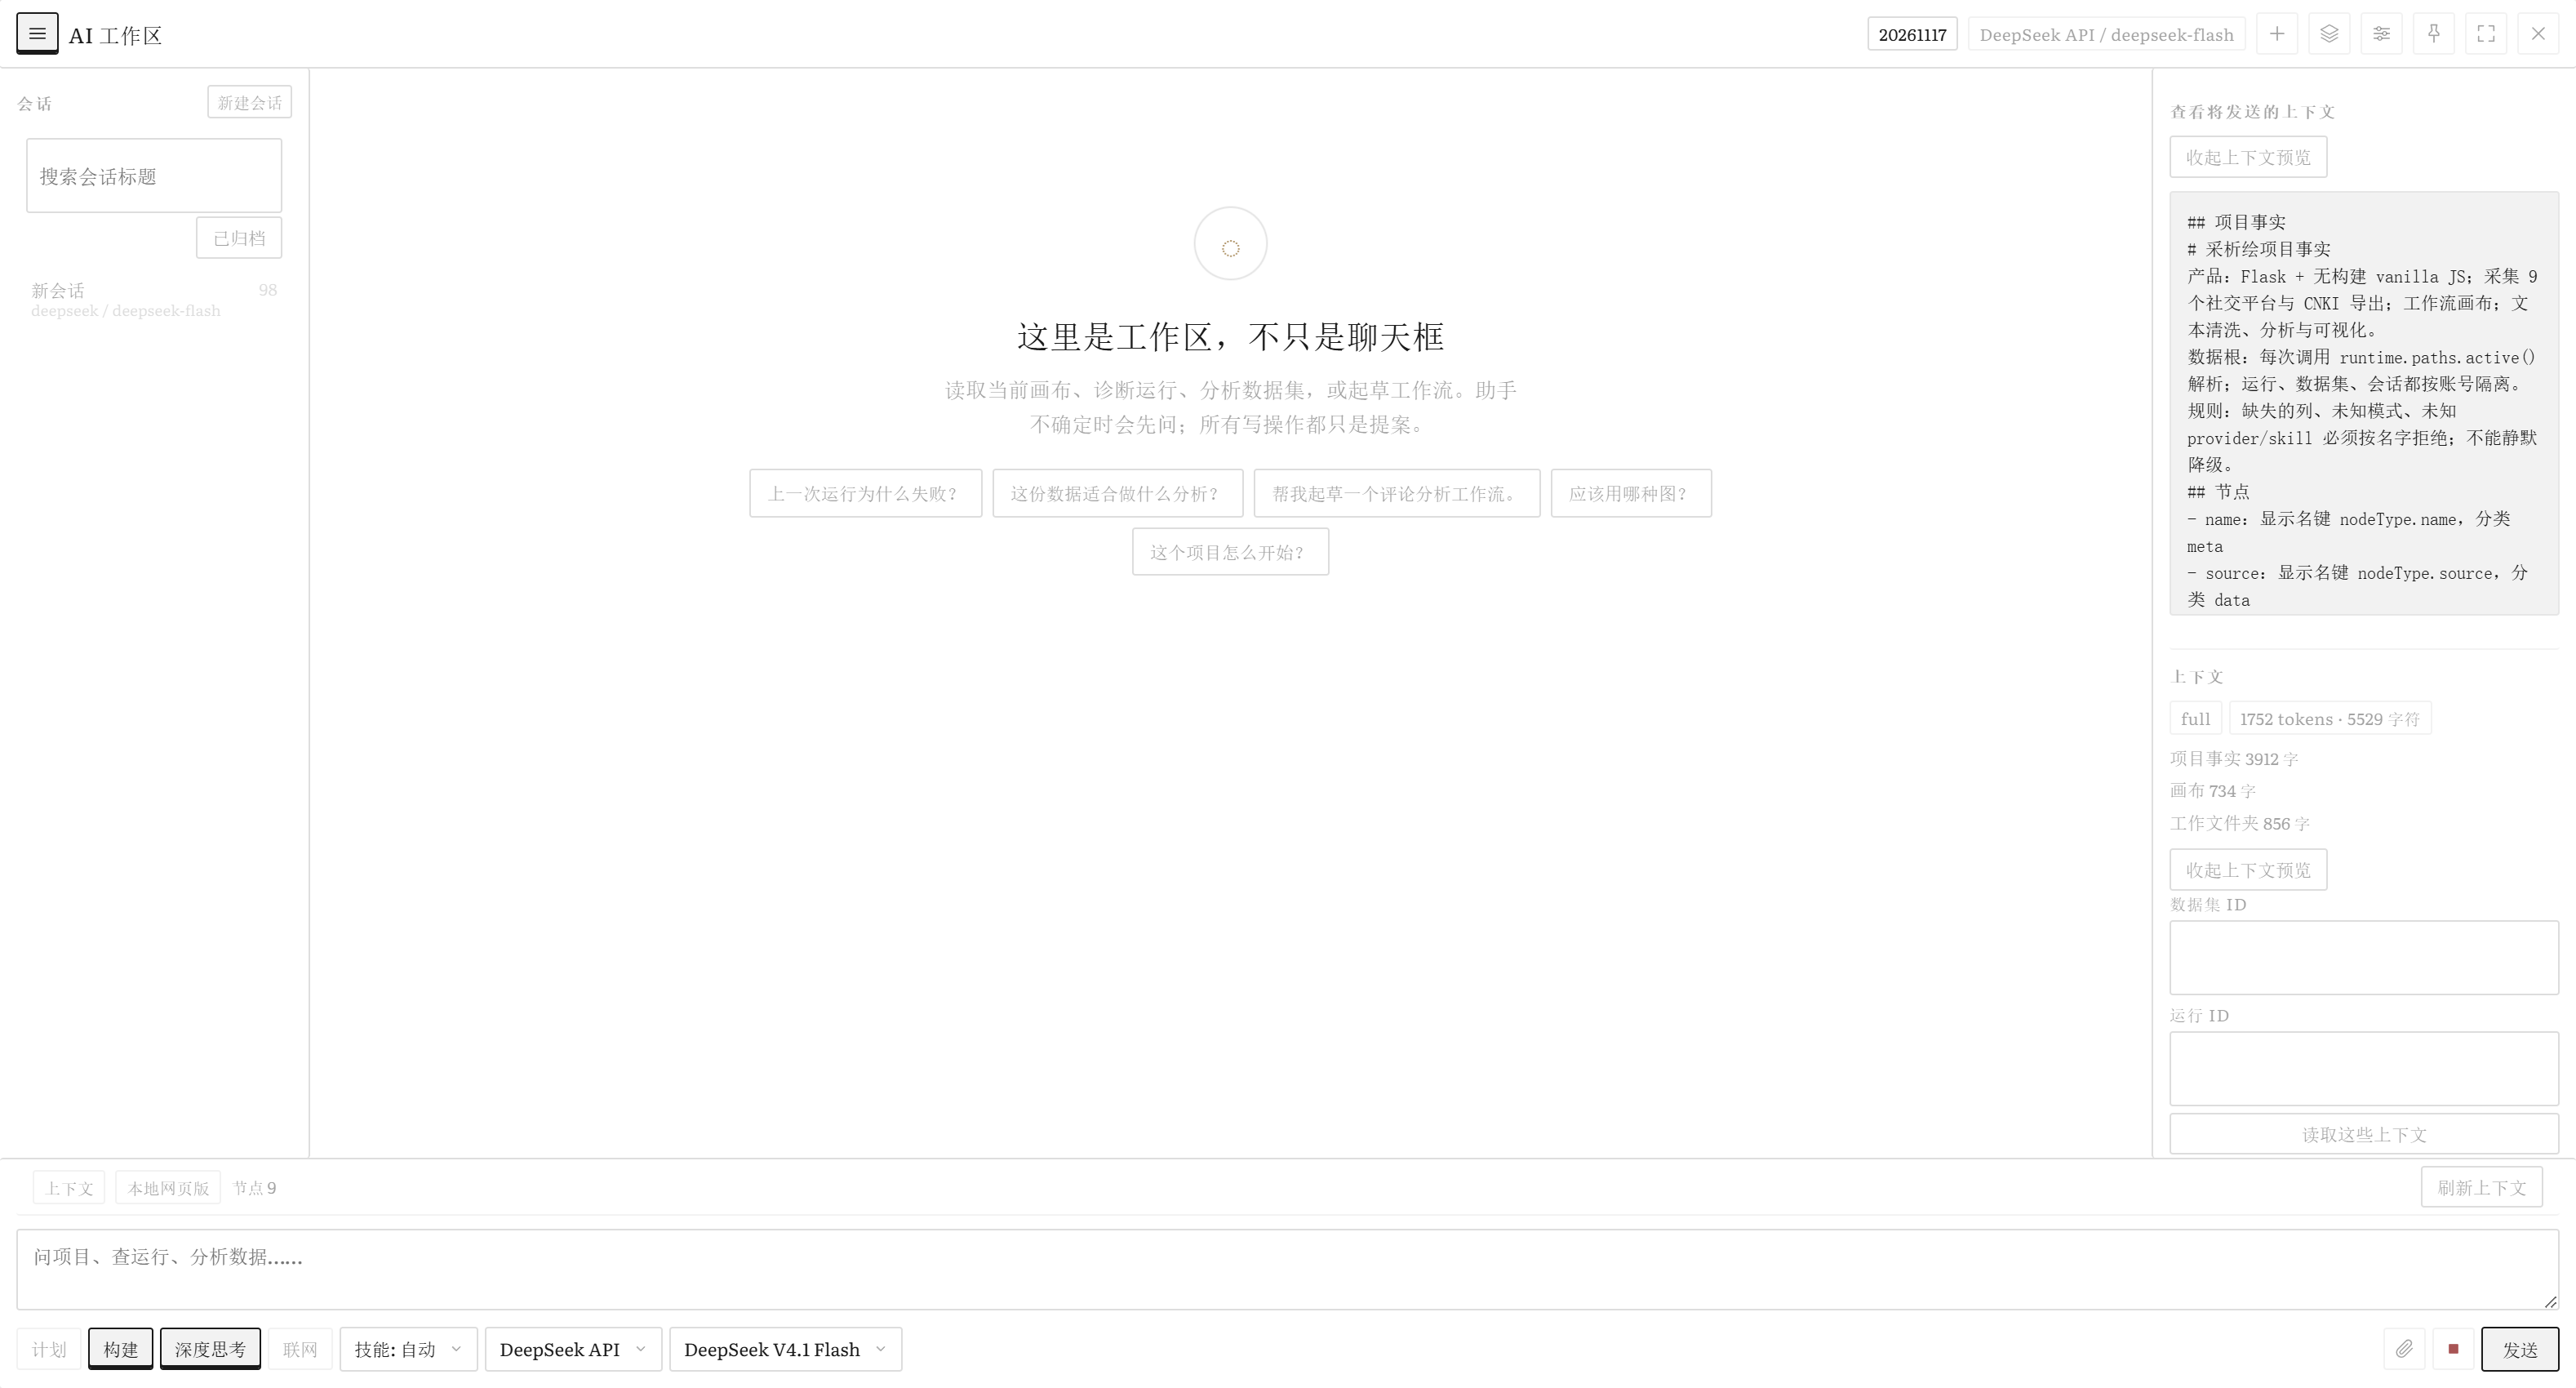
\includegraphics[width=0.98\textwidth]{ai-context.png}
\caption{上下文检查器展示真实文块、token 数字与手动引用框}
\label{fig:ai-context}
\end{figure}

这块内容由服务端生成一次，每个供应商都收到同一份，本地 Ollama 也一样。它以轮的粒度跟着会话走，后面的每一轮原样重放，所以按字节匹配的前缀缓存能一直命中。默认每轮最多重放一万六千字，超出的部分让 AI 用工具现取，检查器会写明已截到多少字。模型窗口也不由服务端放任，到了轮次边界会把最早的几轮裁掉，并写明省略了几条。回答因为输出长度上限被截断时，转录里留一行说明，说继续就能接着写。

输入框里打一个\texttt{@} 可以引用本账号已有的对象。能引的有数据集、导出产物、工作流文件、之前上传过的文件和运行记录。数据集只送列名与前五行，不会把整张表塞进提示词。导出与工作流只展开有界摘要。运行记录给状态、节点错误与控制台尾部。单个附件超过四兆按名字拒绝，并告诉你改走数据集。大表格上传时会自动登记成数据集并给你一个引用。要精确数字，比如多少条、均值、分组汇总、取值分布，就让 AI 用\texttt{dataset\_query}，它是有界的只读聚合，列名不存在或算子不支持都会按名字拒绝，不靠前几行估算。

\subsection{技能与插件}

助手的本领来自技能。顶栏的堆叠图标打开工作室，第一页就是技能与插件。图里列着内置技能，项目向导、采集顾问、故障诊断、运行监控、数据分析、画布架构师、可视化顾问、报告写作、联网研究、Python 扩展、工作区总控和技能作者都在其中。

\begin{figure}[H]\centering
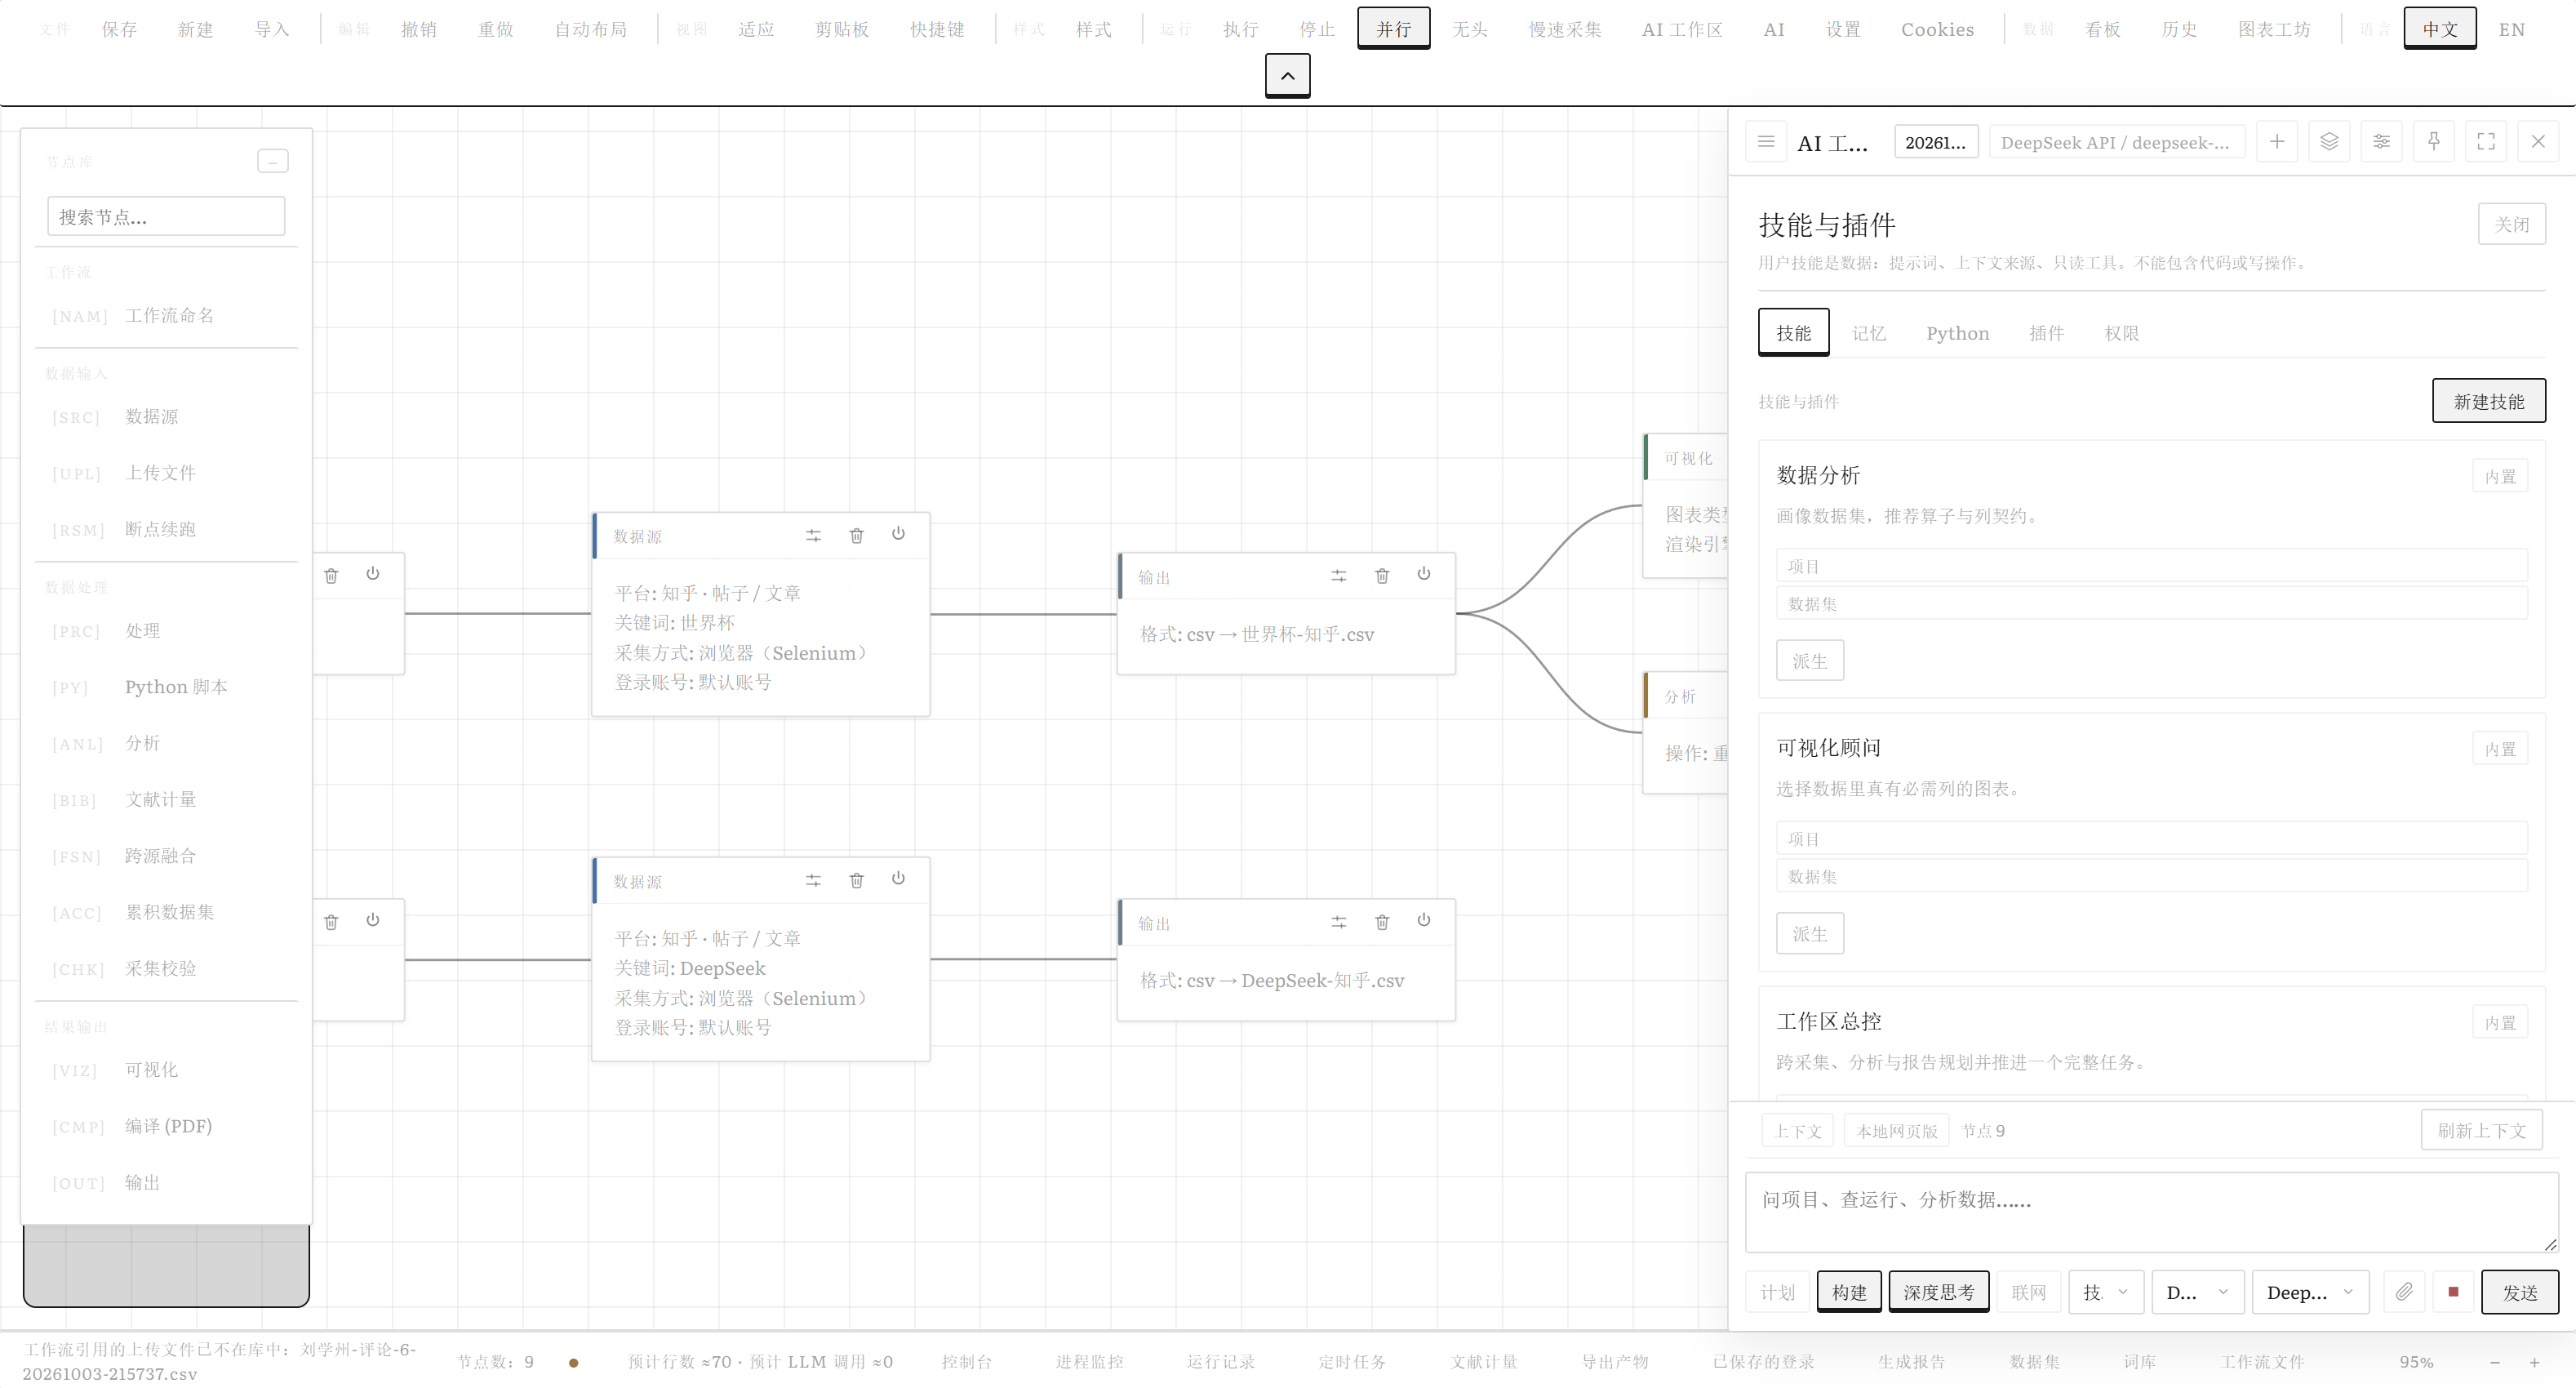
\includegraphics[width=0.98\textwidth]{ai-studio.png}
\caption{工作室技能页，内置技能可派生，用户技能是数据}
\label{fig:ai-studio}
\end{figure}

内置技能只读，可以派生一份再改。用户技能是数据，写的是提示词、上下文来源与允许的只读工具，不能带代码或写操作。插件页装的是声明式技能包、供应商包和工具包。代码插件只允许本机和管理员，云端按名字拒绝。安装是机器级的，使用是账号级的，某个账号装的工具只在这个账号自己的对话里出现。

\subsection{长期记忆}

工作室的记忆页存着你确认过的事实，图里是它空着的样子。助手不能直接写这里。它用一张提案卡说\texttt{记住这条}，你点了才落库。同一句话再存一次会告诉你已经在记忆里。单条超过两千字或者总数超过两百条都按名字拒绝，不会截断也不会悄悄删旧的。

\begin{figure}[H]\centering
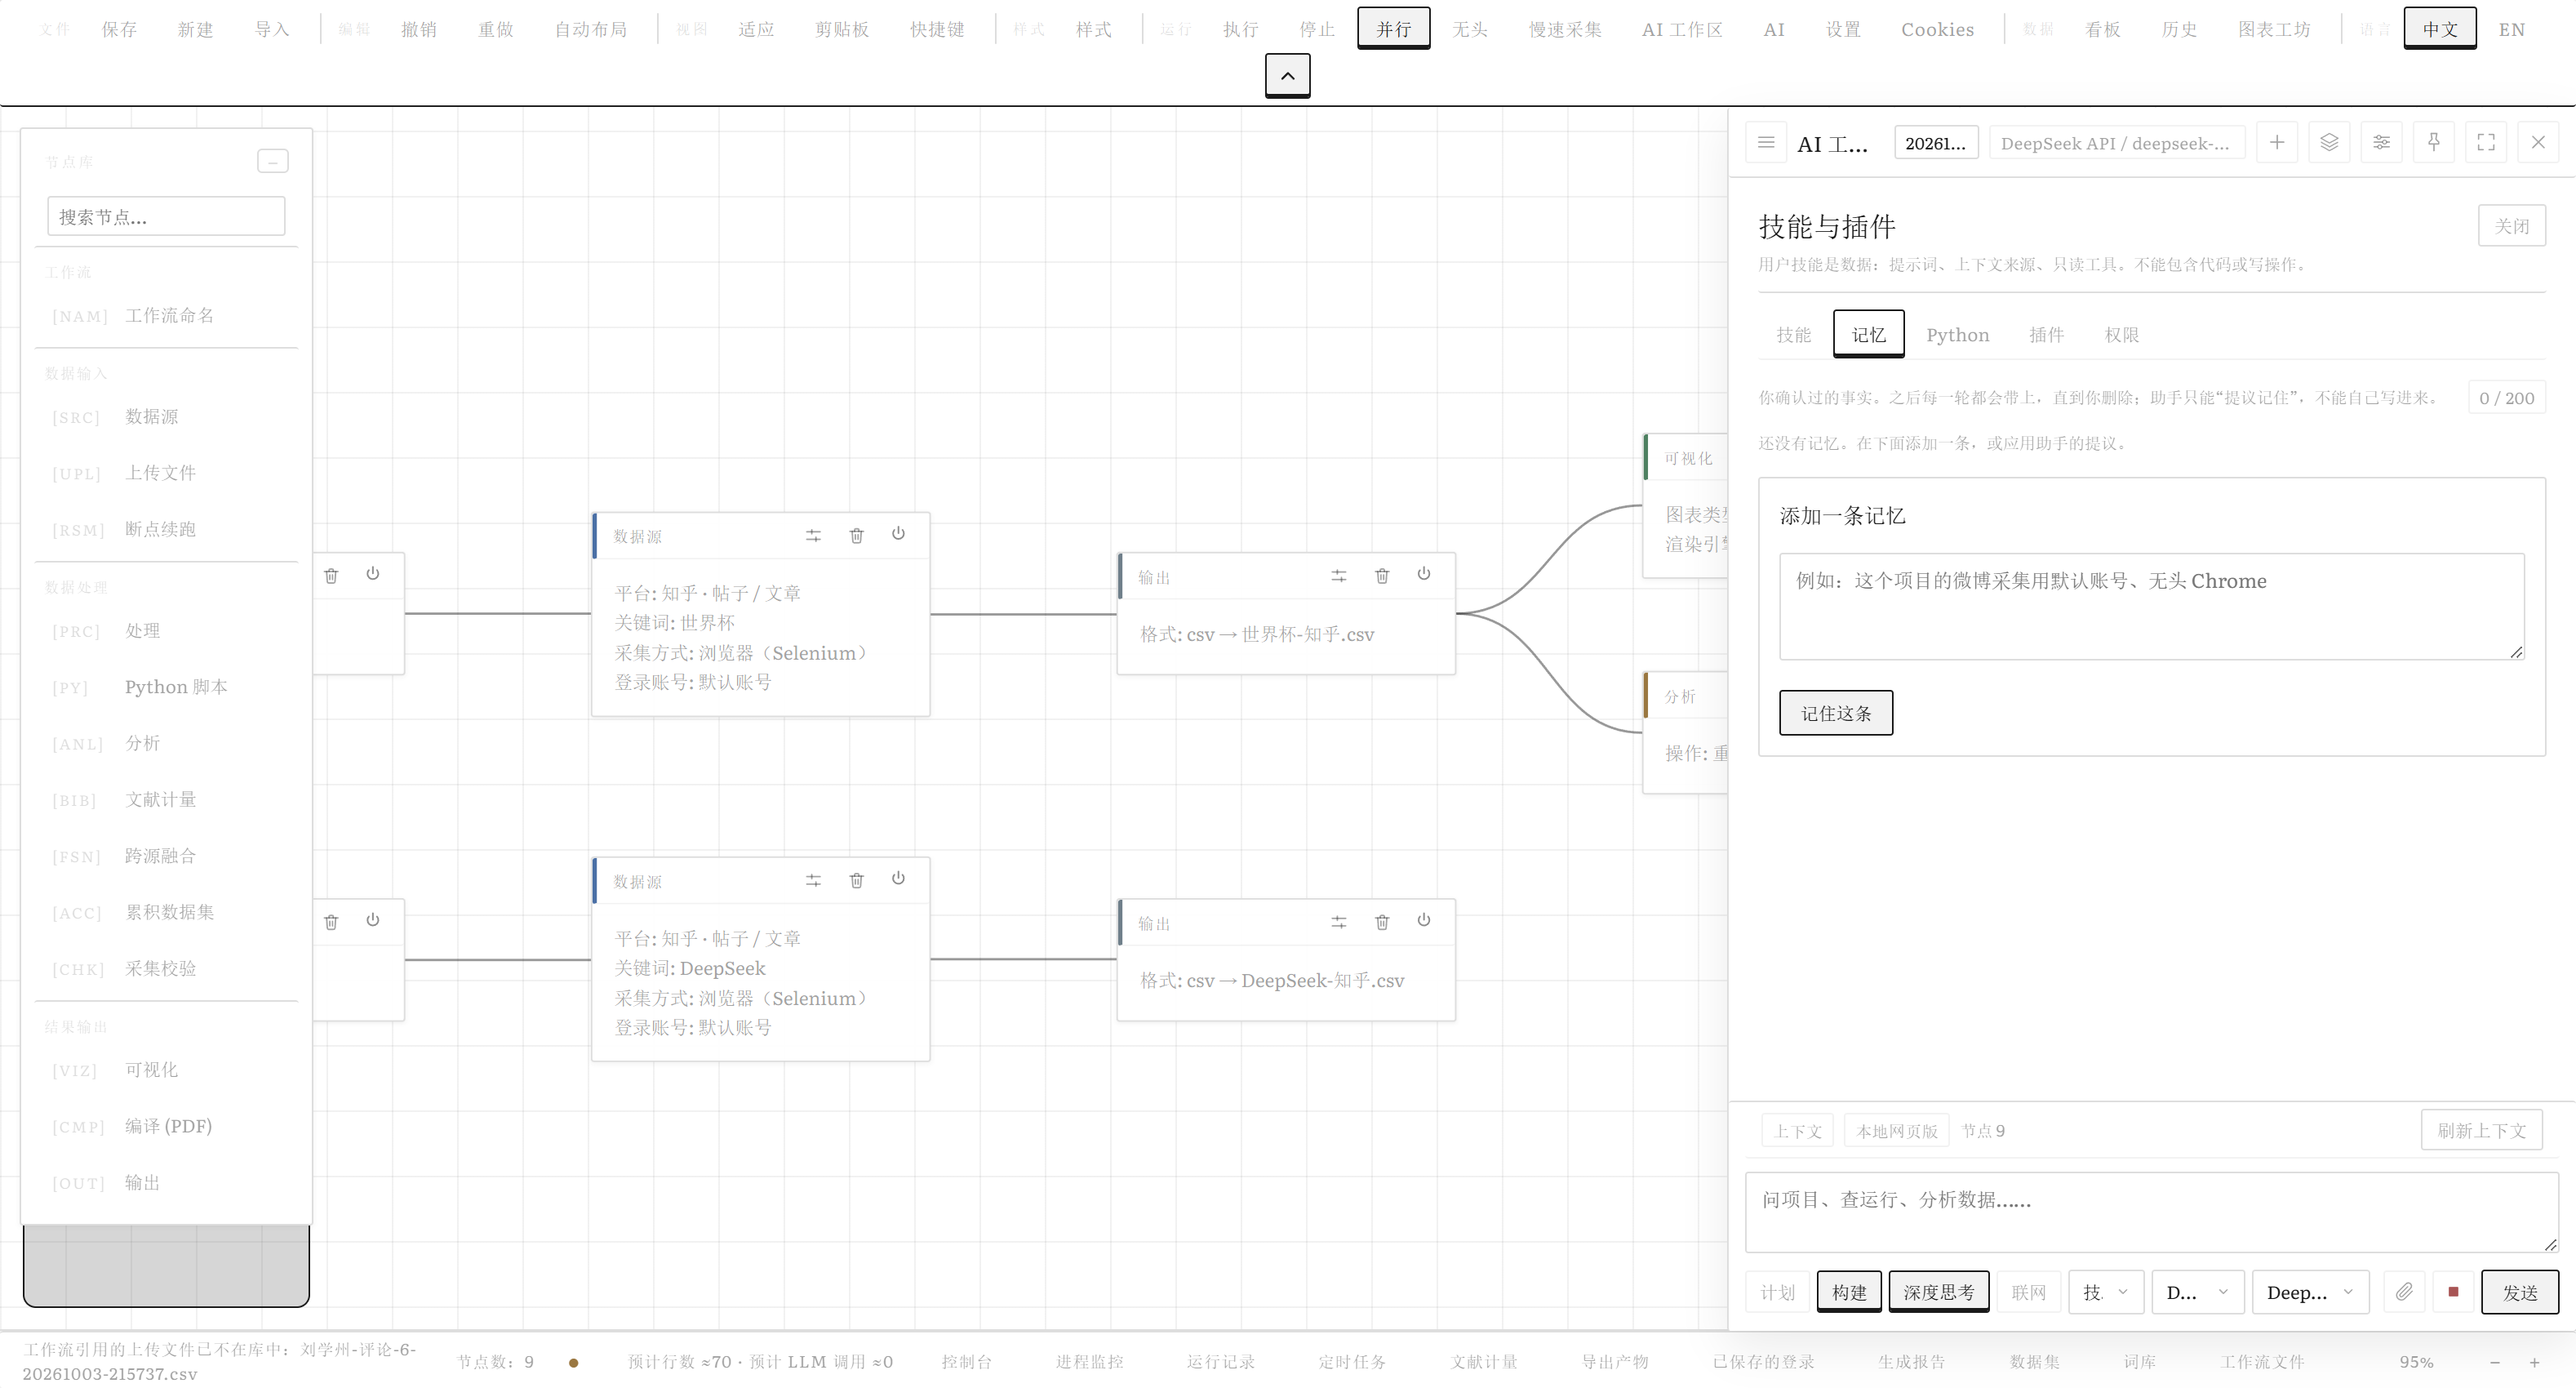
\includegraphics[width=0.98\textwidth]{ai-memory.png}
\caption{记忆页添加一条记忆，助手只能提议不能自己写}
\label{fig:ai-memory}
\end{figure}

每条记忆会跟着之后每一轮的上下文发出去，但只有最新二十条真正进提示词，超出的数量在检查器里写明。记忆随时能删。

\subsection{运行监控与失败重跑}

监控是一条通知渠道，不是一只自己花钱的定时器。你让 AI 提出条件，比如某个节点失败、输出达到多少行、控制台出现某句话、运行结束。它给一张提案卡，你选自动分析或者只通知。运行过程中服务端只在事件流里发布编号、状态和计数，不含爬到的正文。投递写进会话，由浏览器这边处理。自动分析用的是浏览器里那把 Key，服务端自己不花 token。

触发自动分析以后，如果这一轮读到了失败节点，回答里会列出节点编号与错误，下面挂一个\texttt{重跑此节点及其下游}按钮。点它只重跑那一段。它读的是已经保存的工作流文件，要求文件仍与运行记录一致。文件缺失、画布改过、节点不存在、运行还没结束，都按名字拒绝并说清原因。它不会把旧画布载回你当前正在编辑的画布。

\subsection{工作文件夹与本机命令}

桌面版与本地网页版还能让 AI 动你本机的文件。顶栏的工作文件夹那一栏点开，选一个目录。选择窗口列出本机所有磁盘与挂载点，不限于系统盘，也可以点\texttt{用系统窗口浏览}调起系统自带的文件夹对话框。选定以后，AI 能在这个目录里列清单、读写文件、把表格导入成数据集，还能运行一个白名单程序，比如 Python、git、node 与 pytest。这不是 shell，没有管道也没有重定向，所有路径解析后都必须留在那个目录里，越界按名字拒绝。没选文件夹时命令在仓库根或安装根运行。云端不提供这些能力，会按名字拒绝。

动你的东西之前有两道闸。第一道是模式。输入框左边切计划与构建。计划模式下，应用工作流、跑命令、写文件、导入表格这些工具根本不下发，它只能读、校验和给方案。构建模式下才会真的动手并自行核对结果。第二道是逐次审批。关掉自动同意以后，写文件、跑命令、导入表格和重跑节点都不直接执行，AI 必须先提出和它将要做的事完全相同的那一次调用。审批卡显示可核对的预览，写文件给解析后的路径和逐行差异，命令给命令、工作目录与超时，重跑给运行、节点与工作流。预览只读，不会真的写入。你选允许一次、本次会话允许或者拒绝。授权只对这份确切参数有效，换了参数就不命中，拒绝或取消都不授权。

工具轮数默认是三十，到了上限它问你要不要继续，而不是直接失败。单条工具结果默认最多一万二千字，可以在设置里调大。

\subsection{联网搜索与默认值}

工作区默认使用 DeepSeek 直连并默认开启联网搜索：DeepSeek 自 2026-11-18 起，调用模型触发的服务端搜索、抓页工具调用本身免费，结果拼进上下文只按模型 Token 计费。不想联网时从工具栏关掉或在设置里改默认。思考强度可选低、高和最高。非思考轮次的温度默认零点三，让草案与结构化输出更稳。想完全不碰付费接口就打开只用本机模型，开启后选付费供应商会被直接拒绝，不会产生费用。

设置里还能给单会话和当天各设一个 token 软上限，零表示不限。只按真实 token 计，不把不同币种的价格相加。新一轮开始前若已超支，会在写用户消息和调用供应商之前按名字拒绝。一轮之内触顶则借用提问通道问一次继续还是到此为止，答继续只在这一轮生效。本会话用量与余额在检查器里能看，价格未知就说未知，不估算。

\subsection{桌面、网页与云端}

同一套工作区在三端都能用，差别只在宿主能触达什么。判决由服务端给出，前端不猜哪端有什么。

\begin{table}[H]\centering
\caption{三端能用的能力}
\label{tab:ai-hosts}
\small
\begin{tabularx}{\textwidth}{p{4.0cm}XXX}
\toprule
能力 & 桌面版 & 本地网页版 & 云端网页版 \\
\midrule
会话、技能、插件、监控 & 可 & 可 & 可 \\
DeepSeek、OpenCode Go、OpenRouter & 可 & 可 & 可 \\
本机 Ollama 与本机文件 & 可 & 可 & 按名字拒绝 \\
工作文件夹与白名单命令 & 可 & 可 & 按名字拒绝 \\
Python 脚本库、执行与节点 & 可 & 可 & 按名字拒绝 \\
代码插件 & 可 & 可 & 按名字拒绝 \\
\bottomrule
\end{tabularx}
\end{table}

把这一章走完，你已经会让 AI 读上下文、管会话、盯运行、提出方案，也知道写操作为什么要经过你。它不替你选题也不替你下结论，它把重复的查证和草稿接过来，最后一步始终在你手里。
